% !TEX TS-program = lualatex
% !BIB TS-program = biber
%\documentclass[handout]{beamer}
\documentclass{beamer}
\input{../common/misomva}
\newcommand{\misoclasstinytitleslide}{Partially based on material by:  Branislav Kveton, \\[-1em] 
Mikhail Belkin, Jerry Zhu}
\newcommand{\misoclassdate}{}
\begin{document}
% Topic-specific title slide

\newcommand{\topictitle}{Online SSL Applications}

\newcommand{\topicsubtitle}{Face Recognition and Experimental Results}
\renewcommand{\misoclasstinytitleslide}{Partially based on material by:  Branislav Kveton, \\[-1em] Mikhail Belkin, Jerry Zhu}

\MakeTopicSlide

\begin{frame}
\frametitle{SSL with Graphs: Some experimental results}

\begin{center}
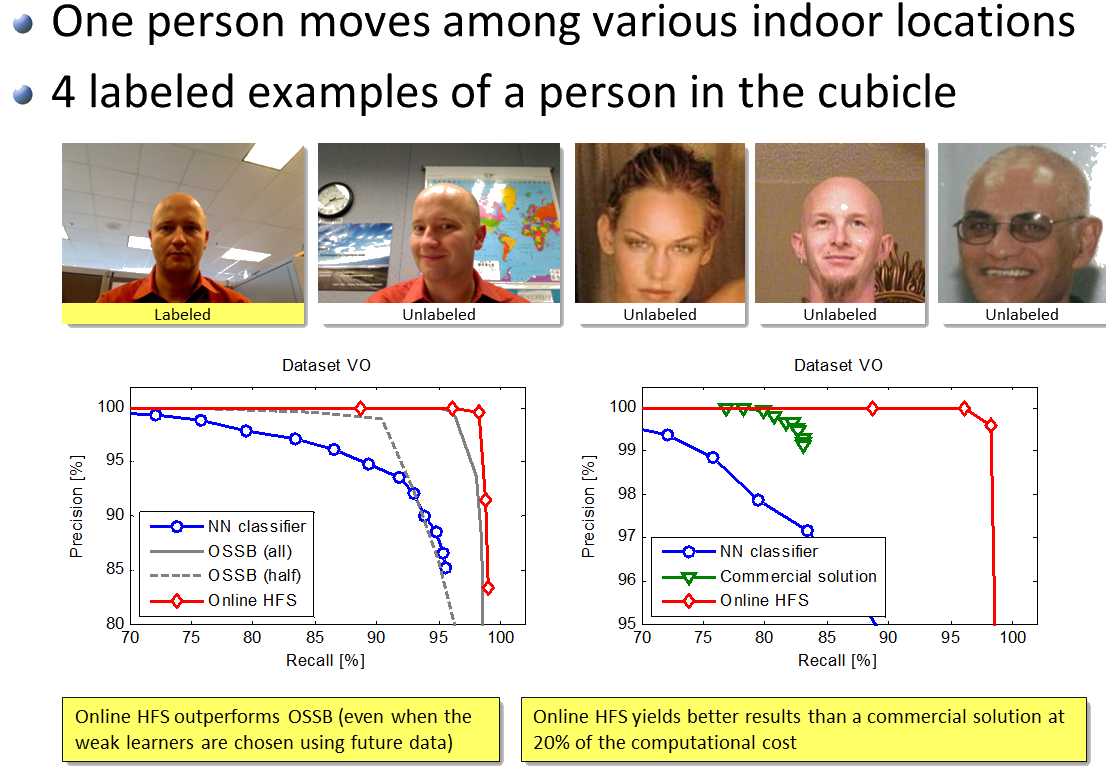
\includegraphics[width=1\columnwidth]{../img/b1}
\end{center}

\end{frame}
%%%%%%%%%%%%%%%%%%%%%%%%%%%%%%%%%%%%%%%%%%%%%%%%%%%%%%%%%%%%
%%%%%%%%%%%%%%%%%%%%%%%%%%%%%%%%%%%%%%%%%%%%%%%%%%%%%%%%%%%%
\begin{frame}
\frametitle{SSL with Graphs: Some experimental results}

\begin{center}
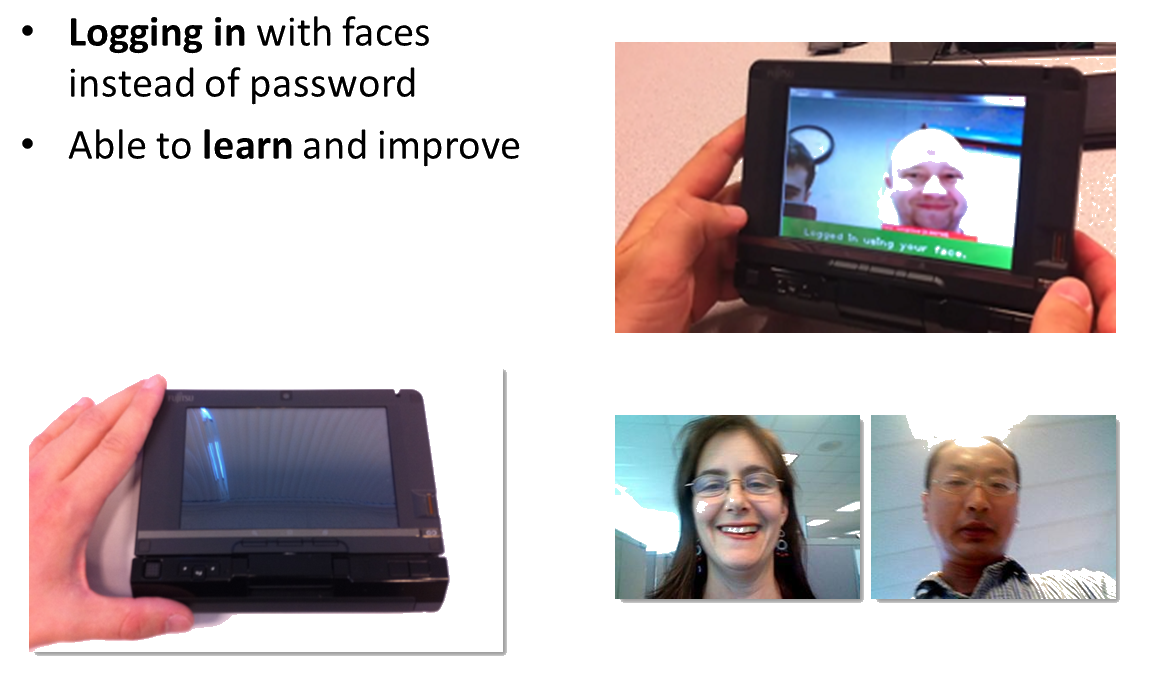
\includegraphics[width=1\columnwidth]{../img/b4}
\end{center}

\end{frame}
%%%%%%%%%%%%%%%%%%%%%%%%%%%%%%%%%%%%%%%%%%%%%%%%%%%%%%%%%%%%
%%%%%%%%%%%%%%%%%%%%%%%%%%%%%%%%%%%%%%%%%%%%%%%%%%%%%%%%%%%%
\begin{frame}
\frametitle{SSL with Graphs: Some experimental results}

\begin{center}
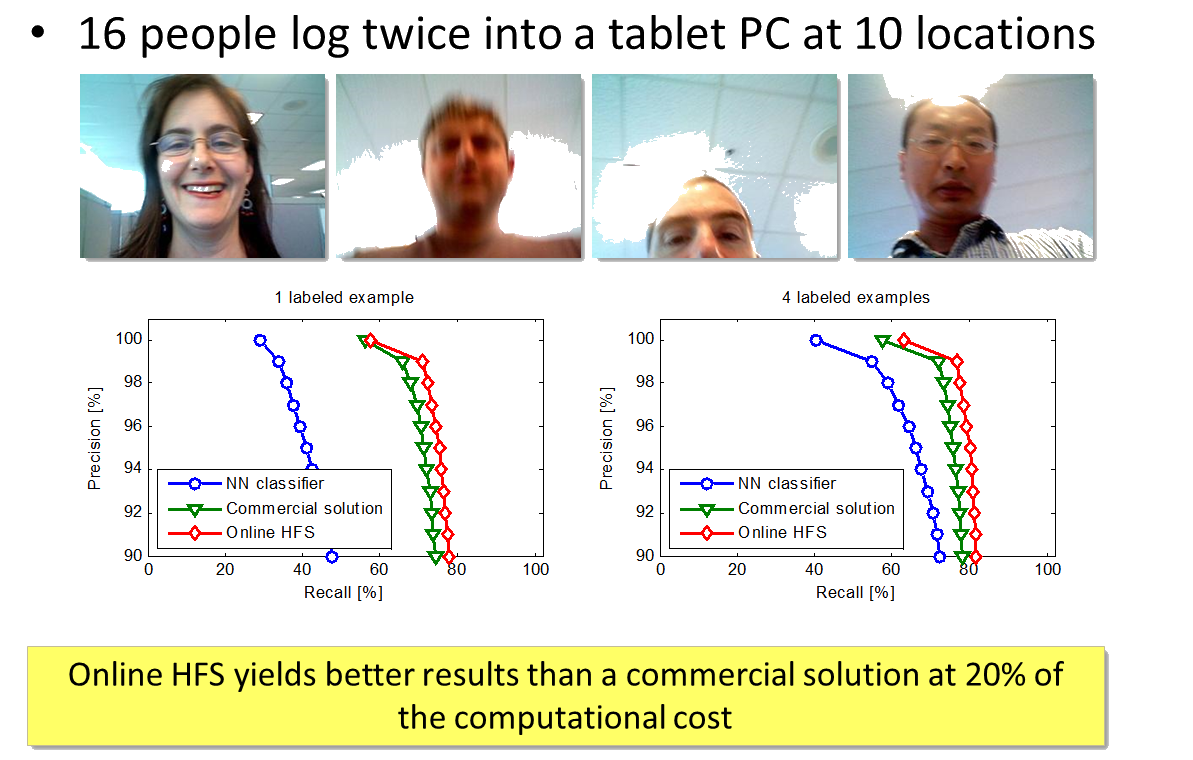
\includegraphics[width=1\columnwidth]{../img/b3}
\end{center}

\end{frame}


\MakeLastSlide
\end{document}
